\begin{center}
    \section*{\fontsize{20}{20}\selectfont Chapter 3}
\end{center}
\vspace{10mm}
\section{Research Methodology}

Write an Introductory passage of Research Methodology here in chapter3.tex

 image sample reference in figure \ref{fig1}
\begin{figure}[htbp]
\centerline{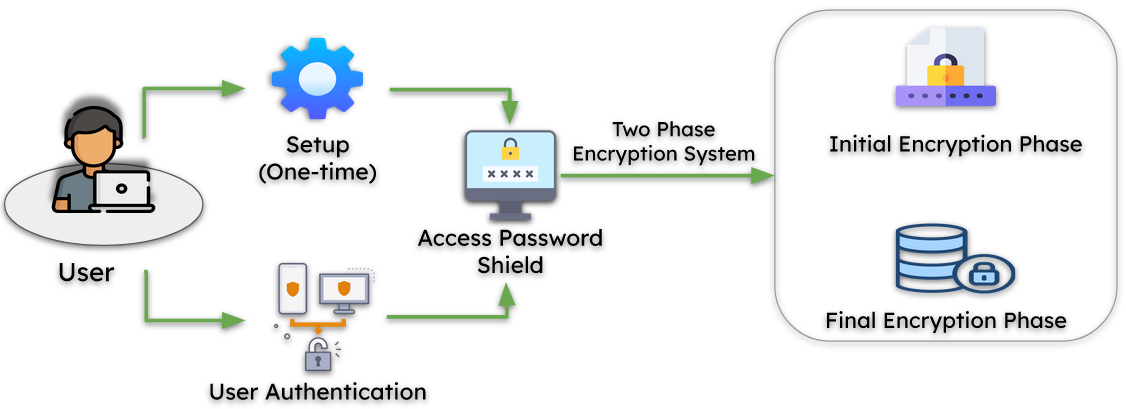
\includegraphics[scale=0.2]{image/method.png}}
\caption{Write proper title of the figure.}
\label{fig1}
\end{figure}

\subsection{Proposed Framework}
Write The Proposed Framework in chapter3.tex

\subsection{Data Set Analysis / Software Project Requirement}
Write the Data Set in chapter3.tex

\begin{table}[htbp]
\caption{Dataset Classes}
\begin{center}
\begin{tabularx}{0.5\textwidth} { 
  | >{\centering\arraybackslash}X 
  | >{\centering\arraybackslash}X 
  | }
\hline
\textbf{-} & \textbf{-}\\
\hline
- & -\\
\hline
- & -\\
\hline
- & -\\
\hline
\end{tabularx}
\label{tab1}
\end{center}
\end{table}

\subsubsection{Subsubsection-1 if necessary}
Write Data Collection \& Prepossessing in chapter3.tex. Write Feature Selection in chapter3.tex

\subsubsection{Subsubsection-2 if necessary}




\subsection{Algorithm/ Model Analysis}
Write the Algorithm in chapter3.tex

\subsection{Explanation of Different Modules}
[if necessary write this segment]
\\
\\
\subsection*{Summary}
Write a Summary passage in chapter3.tex

\clearpage

